\chapter{Background on Operating Systems}\label{ch_background}
\acp{OS} manage the hardware resources - \ac{CPU} time, \ac{I/O} and memory access  - for different tasks and process. 
Dependent on the level of functionalities, \acp{OS} have different levels of complexity.
While a system like FreeRTOS has a limited number of features, Linux offers a variety of services which run in the background. 
\par
This chapter provides a deeper insight into the background of the topic. 
It gives details on \acp{RTOS} in general, on scheduling in FreeRTOS and LinuxRT, and the RT patch. 
Moreover, the causes of \ac{OS} jitter are described, especially the timer interrupt. 
The main design features of real-time programs are discussed and the benchmarking metrics for the two \ac{OS} are introduced. 
Finally, a technique for the estimation of application latency is derived.

\section{The Scheduler}\label{s_scheduler}
Every task or process created by the kernel or a user, is managed by the operating system - more precisely the scheduler. 
It manages all tasks and decides which one is allowed to operate next. 
The decision is based on the priority and the current state of the task. 

\subsection{Task States}\label{ss_task_states}
Dependent on events or resource availability, tasks can enter different states. 
In the following, the state flow (fig. \ref{fig_taskstates}) used in FreeRTOS \cite{freertos} is described. 
The state flow in Linux is related, but extended by other states which are not of interest for further consideration. 

\begin{figure}[htb]
	\begin{center}
		\includegraphics[scale=0.8]{inputs/pictures_ch1/taskstates}
	\end{center}
	\caption[Task State Transitions in FreeRTOS]{Task State Transitions in FreeRTOS with API Calls \cite{freertos}} \label{fig_taskstates}
\end{figure}

\paragraph{Ready}
When a task is schedulable, it is in the \textit{Ready} state.  
A process enters this state when it is first created, has been unblocked by an \ac{ISR} or another task, or when resources it was waiting for become available.

\paragraph{Running}
Tasks in this state get access to the \ac{CPU} as they are currently being executed.
This state can only be entered from tasks in the Ready state.

\paragraph{Blocked}
Tasks enter the \textit{Blocked} state when they are waiting on a queue, a semaphore or another event.
Tasks can switch from this state to the Ready state when the according event occurs, e.g. another tasks releases the semaphore.

\paragraph{Suspended}
A task can be suspended by itself or by another task. 
This task cannot wake up on an event but has to be explicitly unsuspended to reenter the Ready state.  

\subsection{Timer Tick}\label{ss_timer_tick}
The timer tick invokes the scheduler.
Its frequency can be programmed in FreeRTOS as well as in Linux.
The tick is triggered by a timer interrupt a definite number of times per second - the standard on both systems is 100 times. 
On the one hand, processor time might be wasted if a task finishes its execution before the next tick and no context switch is performed.
On the other hand, the \ac{OS} overhead in the system grows if the tick period is too high.
There are no instructions on how to determine the optimum tick period, this is dependent on the specific applications running on that system. 
Programmers can influence the scheduling by calling the \textit{yield} function which invokes the scheduler.
Further, the timer \ac{ISR} is usually used to update the internal system time. 
When no high resolution timer is available, the granularity of the system time depends on the tick.
As the timer tick is implemented in an \ac{ISR}, it causes delays in the system by interrupting the currently executing code. 
Some \acp{OS} provide a configuration called \textit{Tickless kernel} (see fig. \ref{fig_tick}).
It disables the timer interrupt completely when there is no runnable task available to save power as rescheduling is not necessary.
%Jitter in tasks caused by the operating system is called \textit{OS jitter}.

\begin{figure}[htb]
	\begin{center}
		\includegraphics[scale=0.48]{inputs/pictures_ch1/tick}
		\caption[Standard Tick and tickless Kernel]{Standard Tick (left), tickless Kernel (right) \cite{barry:ftssp}} \label{fig_tick}
	\end{center}
\end{figure}

\subsection{Idle Task}
The \textit{Idle Task} is scheduled when no other tasks are present in the Ready queue.
It usually has the lowest possible priority.
This task is often used to put the \ac{CPU} in a low-power mode, e.g. scaling down frequency or executing the \textit{halt} instruction. 
Moreover, it can be used to perform background processes or as indicator for capacity utilization.  
  
\subsection{Scheduling Policies}\label{ss_scheduling_policy} 
The scheduler decides which task will run next by entering the Running state. 
The decision is based on the scheduling policy of the \ac{OS}.
There are mainly two different types of scheduling: \textit{Preemptive} and \textit{cooperative} scheduling.
In cooperative scheduling, tasks cannot be interrupted, they have to release the processor voluntarily. 
Examples for cooperative scheduling are the \textit{\ac{FIFO}} or the \textit{\ac{LIFO}} algorithms.
\ac{RR} or priority based scheduling (\ac{EDF} or \ac{SRTF} algorithm) are examples of preemptive scheduling.
The scheduling policy is crucial for \acp{RTOS} because it determines the handling of real-time tasks.
Obviously, real-time tasks usually have the highest priority and should not be preempted by tasks with lower priority.
For details on scheduling in Linux and FreeRTOS refer to the corresponding sections (\ref{ss_scheduling_in_linux} and \ref{ss_scheduling_in_freertos}).

\section{Intertask Communication and Synchronization}\label{s_intertask_communication}
In \acp{OS}, not only one but many different tasks are usually active.
These tasks need ways to be synchronized with each other.
Race conditions on critical resources, e.g. concurrent memory access, need to be prohibited.

\subsection{Events}
In many cases, tasks need to wait until another task completes execution.
Instead of polling on a resource (actively waiting and therefore wasting \ac{CPU} resources), tasks usually wait for an event to happen.
Therefore, a task blocks or sleeps on a specific signal.
When another task completes execution, it triggers the signal and wakes the task waiting on it.
Such a signal can also be triggered by an \ac{ISR}.
This kind of synchronization can also be realized using semaphores (see \ref{ss_memory_access}).

\subsection{Barriers}\label{ss_barriers}
Sometimes, multiple tasks have to be synchronized at one specific point in the execution flow.
Therefore, all tasks have to wait until the others have finished.
An example is the separation of matrix operations across multiple threads in a multicore system. 
Another example is an application which depends on different data sets collected by multiple threads.
Before the tasks can continue their work, all data has to be available.
Such synchronization points are called barriers.

\subsection{Memory access}\label{ss_memory_access}
Concurrent memory access of multiple tasks can have undesired results as illustrated in the following example (see table \ref{tab_example_concurrent_memory_access}) :\\
Person A and person B want to withdraw money from the same bank account (both 500 Euros) via an ATM at the same time.

\begin{table}[htbp]
	\centering
		\begin{tabular}{|l|l|l|}
			\hline
				Task A 							& Task B 							& Memory  \\
				\hline 
				-- 									& -- 									& X 			\\
			  get X 							& -- 									& X				\\
			  increment X by 500 	& --									& X				\\
			  --									& get X								& X				\\
		 		--		 							& increment X by 500	& X				\\
			  write back X			 	& --									& X	+ 500	\\
			  --									& write back X				& X + 500	\\				   
			\hline
		\end{tabular}
	\caption{Example for concurrent memory access}
	\label{tab_example_concurrent_memory_access}
\end{table}

Task A starts processing the request of person A.
It reads the currently saved value X from memory and subtracts 500 Euros.
At this point, it may run out of time, so task B is scheduled.
Task B also reads the currently stored value X from memory (which has not been updated yet) and subtracts 500 Euros.
Like A before, task B is interrupted at this point and A is scheduled.
Task A writes back the new value X and finishes execution.
Then, B also writes back its value X.
Obviously, the newly written value of X - 500 Euros is wrong, it is supposed to be X - 1000 Euros. 
\par
To prevent such inconsistencies, the memory has to be locked by the accessing task until the correct value has been written back.
So called \textit{mutexes} can be used for this purpose.
When a mutex (short for mutual exclusion) is taken by a task, every other task which tries to access this mutex will be blocked.
By releasing the mutex, the waiting tasks are unblocked.
Mutexes are a special form of semaphores.
Semaphores allow a definite number of tasks to access a particular resource, for a mutex it is limited to one.

\subsection{Priority Inheritance}\label{ss_priority_inheritance}
A problem which may occur while synchronizing memory access for tasks with different priorities is unbounded priority inversion.
This means starving a high priority task by locking specific resources for an indefinite amount of time.
An example is the following situation \cite{rostedt:iotrtp}:
Task A, B and C have different priorities where A has the lowest, B the medium and C the highest priority.
Task A takes mutex M and then is preempted by task B.
Task C attempts to access M as well but is blocked as M is already taken.
Now C is indirectly blocked by B an undefined amount of time, maybe forever, depending on the execution time of B.
\par
This situation can be resolved by priority inheritance.
With priority inheritance, task A gets a priority boost when C tries to access the semaphore.
A inherits the priority of C.
Therefore, task B is preempted by A and A can leave the critical section.
As soon as A releases mutex M, the priority level is set back to normal.
Now C is woken up and can finish its work before B is scheduled again.

\subsection{Message Passing}
One way to exchange information between different tasks is passing messages between each other. 
Usually, one task blocks on a message queue until another task puts a message in this queue.
This event wakes up the blocking task, so it can retrieve the message.
The mechanism is a mix of signaling event and synchronizing shared memory accesses.
It is available in Linux as well as in FreeRTOS.

\section{Interrupt Handling}\label{s_interrupt_handling}
Interrupt signals provide an important method for the processor to communicate with peripheral devices.
The devices range from mice and keyboards to Ethernet or hard drive controllers.
The interrupt signal from a hardware device is connected to the interrupt controller of the processor. 
This controller signals the processor that an \ac{IRQ} has arrived.
Now, as the name suggests, the currently executing process is interrupted, the context saved and the corresponding \ac{ISR} loaded to be executed.
Because they disturb the execution of other processes, \acp{ISR} should be kept as short as possible.
The minimal version of an \ac{ISR} should at least contain the acknowledge of the interrupt so the underlying hardware can continue its work.
The time between an interrupt being triggered and the first instruction of the corresponding \ac{ISR} is called interrupt latency.
Typically, only urgent operations are performed in an \ac{ISR}. 
For less critical work, e.g. handling incoming data from a network device, an extra routine is started which can be run later.
This mechanism is referred to as division of the interrupt management in two halves: A \textit{top half} (\ac{ISR}) and a \textit{bottom half} (deferred work).
The implementation of the bottom half is dependent on the operating system. 
\par
Interrupts can occur any time and are serviced immediately.
Consequently, any code currently running will be interrupted.
Some sections in the kernel code have to be run without interruption to prevent critical errors in the systems.
Such sections are called critical sections.
Interrupts are usually disabled on entering a critical section.
Therefore, servicing the interrupt is postponed what causes a higher interrupt latency.
Interrupts can be prioritized what enables interrupt nesting.
This causes high priority interrupts to disturb the execution of lower prioritized interrupts.
 
\section{Hardware Delays and \ac{OS} jitter}\label{s_hardware_delays_and_os_jitter}
Different delays caused by the underlying hardware or the \ac{OS} are crucial in real-time applications.
In this work, the term \textit{delay} refers to unexpected events which extend the mean execution time of a real-time task.
The maximum delay is also referred to as jitter.  

\begin{figure}[htb]
	\begin{center}
		\includegraphics[scale=0.8]{inputs/pictures_ch1/delay}
	\end{center}
	\caption[Delay in Task caused by Interrupt]{Delay in Task caused by Interrupt} \label{fig_delay}
\end{figure}

In contrast, \textit{latency} is the time a real-time task or a piece of code actually needs to execute. 
There are mainly three kind of delays and one kind of latency:
\begin{enumerate}
	\item Delays from the Operating System
	\item Delays from interrupts (fig. \ref{fig_delay})
	\item Delays from cache misses
	\item Latencies from task execution and synchronization
\end{enumerate}
Moreover, the boot time can be crucial in special real-time application.

\subsection{Delays from the Operating System}
The obvious kind of delay which is inevitable when using an \ac{OS} is the delay caused by the \ac{OS} itself.
The most significant (and predictable) delay is caused by the timer tick.
More delays can be produced by background daemons and other system services. 

\subsection{Delays from Interrupts}
The second kind of delays (for details refer to \ref{s_interrupt_handling}) can only be prevented by introducing critical sections. 
However, this may cause higher interrupt latencies and is counterproductive in applications which rely on fast interrupt response times.
In Linux, critical sections can only be found inside of the kernel.
If interrupts should be disabled in user mode, this is only possible by calling a device driver routine which implements the disabling and enabling of interrupts.  
As interrupts are mainly caused by \ac{I/O} devices, the delays from interrupts will increase when the system heavily communicates with a large number of peripherals. 

\subsection{Delays from Cache Misses}
The last cause of delays is caching.
Caches are fast buffers which allow faster data access to data currently cached.
They are often built up hierarchical (level 1, level 2, ...) and divided into data and instruction caches.
A typical set up are separate level 1 data and instruction caches for each \ac{CPU} and a shared level 2 cache for both data and instructions for all \acp{CPU}.
On the one hand, caches increase the performance of an application significantly by reducing slower memory accesses to the \ac{RAM}. 
On the other hand, the cache is used by every process on the system.
This can cause data currently needed by a real-time application not to be present in the cache, a cache miss occurs.
The reload of the data to the cache causes a delay.
The delay is hardware dependent. 

\subsection{Latencies from Task Execution and Synchronization}
The last aspect is more correctly defined as latency, not as delay.
It specifies the time which is caused by using the synchronization methods provided by the \ac{OS}. 
These latencies are implementation specific.
Their execution time can be measured.
\par
The obvious one is the task switching time when a context switch occurs.
This is not avoidable and happens either when the timer tick occurs (refer to \ref{ss_timer_tick}), a task blocks, finishes or voluntarily releases the \ac{CPU}.
Another latency related to scheduling is the preemption time.
This is the time which it takes the \ac{OS} to interrupt a low priority task and schedule a high priority task.
The rescheduling can be caused by giving a semaphore, sending a message or waking up a high-priority task from an \ac{ISR}.
\par
Moreover, task synchronization causes latencies in a \ac{OS}.
Examples are semaphores, mutexes, message passing or signals. 
When a mutex is released, other tasks may be unblocked.
This means, that whenever this action happens, the \ac{OS} has to check whether tasks can be moved from the Blocked state to the Ready state.
If a task with higher priority has been woken up, the current task is preempted and a context switch takes place.
Dependent on the application and the right synchronization mechanism, the overall system latency can be reduced.
\par
The latencies described in this section are \ac{CPU} bound compared to \ac{I/O} bound delays which are caused by interrupts.
 
\subsection{Boot Time}\label{ss_boot_time_general}
The boot time can be a relevant factor for the choice of a specific \ac{OS} if the system needs to start up very fast.
When a car is started, the driver does not want to wait 15 seconds until the ignition starts running.
\par
The boot time depends on the memory print of the operating system and the medium from which the \ac{OS} is loaded.
Another important factor is the initialization of hardware structures, e.g \ac{FPGA} designs.
Moreover, a file system may be needed for the \ac{OS} kernel to work properly which must be loaded besides the actual kernel. 
A boot loader is necessary to start an application or an \ac{OS}.
\par
For simple programs or light-weight \ac{OS} like FreeRTOS a \ac{FSBL} is usually sufficient.
This can as well optionally load an \ac{FPGA} design.
For more complex systems like Linux \cite{jones:itlbp}, the \ac{FSBL} is used to load a more sophisticated \ac{SSBL}.
Then the \ac{SSBL} loads the kernel and optionally the initial RAM disk image and a hardware initialization file (device tree) into memory.
After those steps, the kernel can be decompressed and finally boot.
While booting, it initializes the file system with the previously loaded image, the peripheral devices and finally starts the user space applications. 
\par
Ways to optimize this process will be discussed later (refer to section \ref{s_boot_time}).

\section{FreeRTOS}
This section describes the \ac{OS} FreeRTOS in more detail.
The focus is on the scheduling algorithm, interrupt handling and synchronization features.

\subsection{Scheduling in FreeRTOS}\label{ss_scheduling_in_freertos}
Scheduling in FreeRTOS \cite{freertos} can be either cooperative or preemptive and is purely priority based.
The maximum priority can be defined by the user. 
The memory footprint grows with increasing priority number, so it is recommended to choose only as many priority levels as needed.
The task with the highest priority which is in the Ready state will be scheduled. 
Tasks can have the same priority if desired.
Priorities can be changed during runtime.
\par
All tasks are managed in doubly linked lists dependent on their state (see fig. \ref{fig_freertos_ready_queue}). 
The Ready state is implemented as a list array indexed by the priority level. 
When the scheduler is invoked, it first updates the Ready lists and then schedules the next task.
In case there are multiple tasks in one list, the \ac{RR} algorithm is used to pick the next one.

\begin{figure}[htb]
	\begin{center}
		\includegraphics[scale=0.8]{inputs/pictures_ch1/freertos_ready_queue}
	\end{center}
	\caption[FreeRTOS Ready Queue]{FreeRTOS Ready Queue \cite{dev:taoosa}} \label{fig_freertos_ready_queue}
\end{figure}

\subsection{Interrupts in FreeRTOS}\label{ss_interrupts_in_freertos}
FreeRTOS itself contains only one interrupt: The timer tick (refer to section \ref{ss_timer_tick}).
Other devices and interrupts may be installed on demand, but they are not handled by the OS. 
It is only in charge of task managing and inter-task communication.
For the application development, it means that an interrupt handler has to be written and registered in the interrupt controller.
As all interrupt handling is up to the programmer, it is easy to keep track of the number of interrupts in the system.

\subsection{Synchronization Features in FreeRTOS}
In this section, a short overview of the FreeRTOS \ac{API} features is given.
Most \ac{API} functions are implemented for the usage in tasks as well as in \acp{ISR}.
FreeRTOS uses different kind of semaphores and message queues as synchronization features.

\subsubsection{Tasks and Co-routines}
Every FreeRTOS application is structured as a set of tasks and/or co-routines.
Each task is provided with its own stack where the current processor context is saved on a task switch.
Tasks are fully prioritized, support full preemption and are not restricted in usage.
Co-routines, on the other hand, share a stack within the same application. 
This reduces their amount of \ac{RAM} needed but requires special considerations and restrictions in implementation (for more details refer to \cite{freertos_coroutines_tasks}).

\subsubsection{Semaphores}
FreeRTOS supports three kind of semaphores:
\begin{itemize}
	\item Binary Semaphores
	\item Mutexes
	\item Counting Semaphores
\end{itemize}
All semaphores support priority inheritance.
The implementation is based on message queues.
Mutexes and counting semaphores correspond to the memory access synchronization tools mentioned above (see section \ref{ss_memory_access}). 
These semaphores need to be given back once taken.
Binary semaphores are used as signals for event synchronization.
In contrast to counting semaphores and mutexes, binary semaphores are taken by the task which is waiting for an event and given by the signaling task. 

\subsection{Booting in FreeRTOS}\label{ss_booting_in_freertos}
The booting process of FreeRTOS consists of booting the \ac{ROM} file, loading and running the \ac{FSBL}, optionally loading a bitstream and finally loading and running the application (compare to figure \ref{fig_boot_freertos}).
There is barely room for optimization in the first two steps of the booting process. 
However, the last two steps are dependent on the size of the bitstream and the size of the application respectively.

\section{LinuxRT}
This section describes the Linux \ac{OS} in more detail.
The focus is on memory management, the scheduling algorithm, interrupt handling and synchronization features.
Moreover, the differences between the mainline Linux kernel and the RT patch are explained.

\subsection{Memory Management}
%The Linux \ac{OS} uses a quite complex system 
Linux uses a file system to store user programs and system data. 
This file system is usually larger than the available \ac{RAM}, therefore it is provided on an other medium.
The medium can be for instance a removable flash disk like an \ac{SD} card, a \ac{QSPI} flash or a hard drive.
Because it provides much faster data access, the \ac{RAM} is much more expensive and usually smaller than the other medium. 
For faster data access, program data stored in the file system is loaded dynamically from hard disk into \ac{RAM} during run time.
This is called mapping physical memory (from the file system) to virtual memory (\ac{RAM}).
Because of efficiency considerations, the data blocks are managed in pages of consequent data which usually consist of several kBs.
The pages used by a real-time application could be flushed from the \ac{RAM} which causes hardly predicable delays when reloading the pages.
Yet, there is the possibility to lock specific pages for critical applications in \ac{RAM}.
This feature should be used carefully because it might increase the run time of one application but decrease the over-all system performance by blocking the \ac{RAM}.   

\subsection{Scheduling in Linux}\label{ss_scheduling_in_linux} 
Scheduling in Linux \cite{love:lkd} \cite{jones:itlcfss} is more complex than in FreeRTOS.
Three scheduling classes are used to determine which task will be selected: \textit{sched\_rt}, \textit{sched\_fair} and \textit{sched\_idletask}.
Sched\_rt implements the scheduling of real-time tasks and has the highest priority. 
General purpose tasks are using the sched\_fair class and the remaining class is used by the idle task (see fig. \ref{fig_linux_scheduling_classes}).

\begin{figure}[htb]
	\begin{center}
		\includegraphics[scale=0.6]{inputs/pictures_ch1/linux_scheduling_classes}
	\end{center}
	\caption[Linux Scheduling Classes]{Linux Scheduling Classes \cite{jones:itlcfss}} \label{fig_linux_scheduling_classes}
\end{figure}

\subsubsection{sched\_rt} 
Linux real-time tasks are always scheduled prior to any other task. 
The default priority levels range from 0 to 99 where 99 is the highest possible value.
The maximum priority can be configured by the user. 
The run queue is implemented comparable to the one of FreeRTOS. 
In Linux, there are two different scheduling policies for real-time tasks: \ac{RR} (preemptive) and \ac{FIFO} (cooperative).

\subsubsection{sched\_fair}
For the sake of completeness, the fair scheduling algorithm is briefly described in this section.
Linux was originally developed as a General Purpose \ac{OS}, so its scheduling algorithm is optimized to treat all tasks as fair as possible. 
The current scheduler is called \textit{\ac{CFS}} and was introduced in Linux kernel 2.6.23.
It is implemented as a Red-Black tree (see fig. \ref{fig_linux_red_black_tree}), which is self-balancing (no path is more than twice as long as any other).
An element of the tree can be accessed in in O(log n), where n is the total number of nodes in the tree.
\begin{figure}[htb]
	\begin{center}
		\includegraphics[scale=0.88]{inputs/pictures_ch1/linux_red_black_tree}
	\end{center}
	\caption[Example of a Red Black Tree]{Example of a Red Black Tree \cite{jones:itlcfss}} \label{fig_linux_red_black_tree}
\end{figure}
The prioritization of the \ac{CFS} is based on the time the tasks have already been executed. 
The lesser the time compared to the other tasks, the higher the chance to get \ac{CPU} access.
The most-left node is scheduled on a context switch.
Further, the priority of an element can be influenced using the \textit{nice} command. 
It puts a weight on the according node which will change the priority relative to the other nice values.

\subsection{Interrupts in Linux}\label{ss_interrupts_in_linux}
The interrupt handling in Linux is integrated into the operating system.
Each hardware device needs a driver to communicate with the \ac{OS}.
This driver provides \textit{open()}, \textit{read()} or \textit{write()} functions to access the device. 
It has to be registered before the device can be used.
Drivers can be started at boot time or dynamically be loaded as modules during runtime.
The interrupt handler is part of the driver and has to be registered in the kernel by calling the function \textit{irq\_request()} and deregistered by calling \textit{irq\_free()}.
When an interrupt occurs (compare figure \ref{fig_irq_path_linux}), the \textit{do\_IRQ()} kernel function is called which takes care of all \acp{ISR}. 
Interrupt handler cannot be implemented by a user application.
Applications running in user mode have to use read, write or \ac{I/O} control functions to access the specific device.
\begin{figure}[htb]
	\begin{center}
		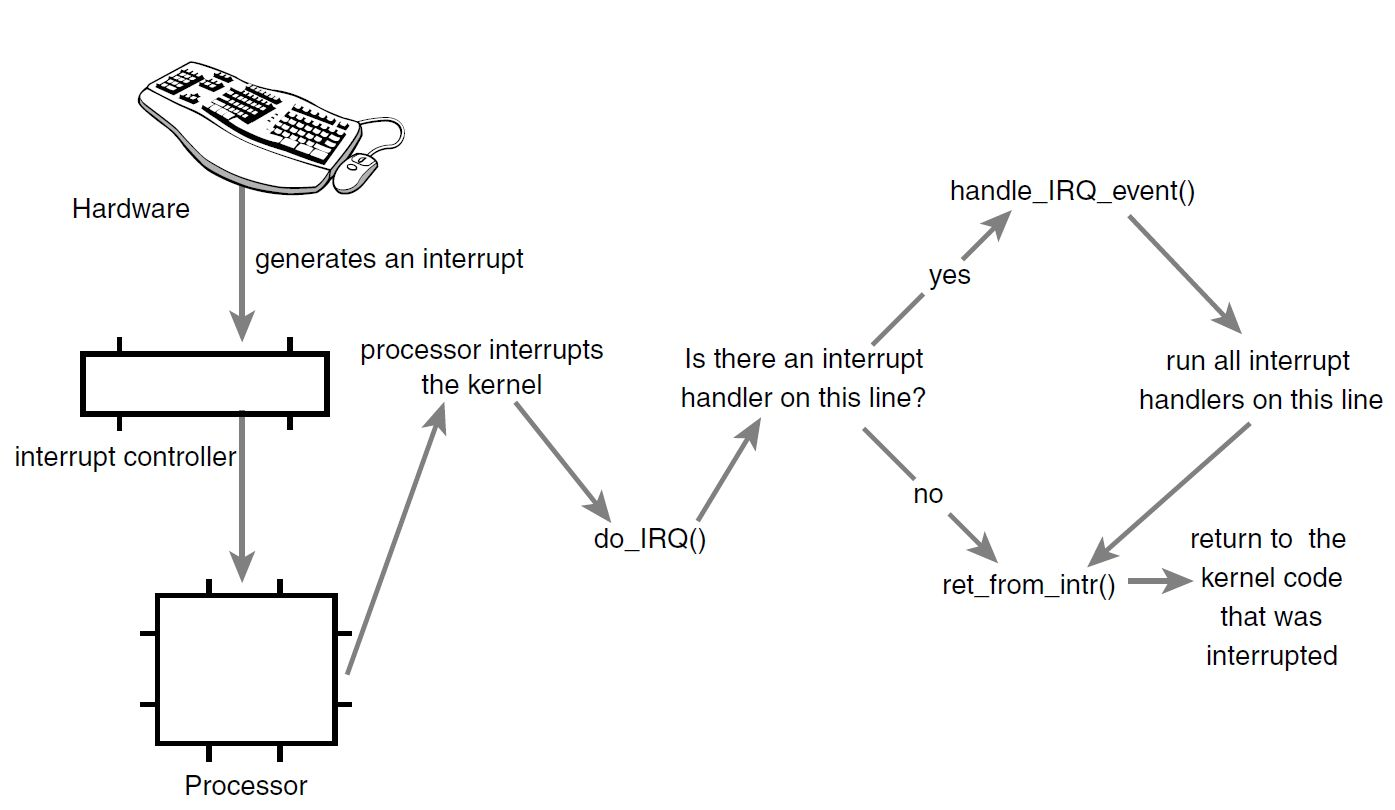
\includegraphics[scale=0.3]{inputs/pictures_ch1/irq_path_linux}
	\end{center}
	\caption[Path of an Interrupt from Hardware through the Kernel]{Path of an Interrupt from Hardware through the Kernel \cite{love:lkd}} \label{fig_irq_path_linux}
\end{figure}

Further, it is typical in Linux to defer non-critical work from the \ac{ISR} to a bottom half.
There are multiple types of bottom halves in Linux, the most important are \textit{softirqs} and \textit{tasklets} \cite{love:lkd}.
Softirqs are statically registered in the kernel during compile time and are only interruptible by \acp{IRQ}.
Their number is limited by the \ac{OS}.
In standard Linux they are invoked when the system is returning from a hardware interrupt, in the \textit{ksoftirqd} thread or by an explicit function call to \textit{do\_softirq()}.
Softirqs - even the same type - can run concurrently on multiple \acp{CPU} but cannot interrupt other softirqs.
Usually, all raised softirqs are handled by the do\_softirq function, but when too many softirqs are pending, they are moved to the ksoftirqd thread which is scheduled when the \ac{OS} is not busy.
\par
Tasklets are built on top of softirqs and are not related to tasks as the name may suggest. 
Compared to softirqs, tasklets have a lighter interface.
Further, tasklets of the same type cannot run concurrently, even on different \acp{CPU}.
Moreover, they can be created dynamically during run time.
\par
Another option to defer work is to use to a work queue.
Work queues schedule kernel threads and can sleep if necessary compared to the other two options

\subsection{Synchronization Features in Linux}\label{ss_sync_features_in_linux}
Linux provides multiple \acp{API} with a variety of task synchronization features. 
\ac{POSIX} compliant features are most common because of their compatibility across many platforms.
\subsubsection{Processes and Pthreads}\label{sss_processes_and_pthreads}
A program which runs in Linux is called a process. 
Each process has an own process ID and maintains its own stack. 
The usual way to create multi-tasking systems in Linux is by using so called \textit{pthreads}.
pthreads are light-weight processes which have their own stack but share the parent's virtual memory and environment \cite{barney:pthreads}.
A thread can be created with less cost compared to a process.
Moreover, inter-thread communication is more efficient and is often easier to use than inter-process communication.
pthreads can be prioritized and scheduled individually. 

\subsubsection{Semaphores}
In Linux, there are similar kind of semaphores compared to FreeRTOS.
The \ac{POSIX} \ac{API} provides access to counting semaphores which are referred to simply as semaphores.
Further, mutexes can be used on their own and in combination with condition variables.
Condition variables provide a way to notify a specific thread when an event has occurred. 
On initialization, attributes can be passed to semaphores and mutexes.
The attribute determines for example whether a mutex supports priority inheritance or not.

\subsubsection{Barriers}
Barriers are a very convenient and powerful way of synchronizing threads. 
The \ac{API} provides conventional barriers as described above (see \ref{ss_barriers}) and the \textit{join} function.
The difference between the two is that the barrier synchronizes multiple running threads but the join function allows only one thread to wait for the termination of another.
The result of join is undefined when multiple threads call the join function on the same thread.

\subsection{Booting in Linux}
The Linux booting process is more complex than the FreeRTOS one (see figure \ref{s_boot_time}). 
Linux uses not only an \ac{FSBL} but also a \ac{SSBL}.
Moreover, Linux needs a file system and a device tree to run.
The device tree has to be loaded during booting and provides information on hardware initialization.
If an \ac{FPGA} design is included in the system, it has to be loaded as well.
\par
All these factors have an impact on the boot time and there are different configuration alternatives to initialize the \ac{FPGA} or to load the file systems (see \ref{ss_booting_in_linux} for more details). 

\subsection{RT patch vs. standard kernel}
The Linux RT patch aims to make the Linux kernel more preemptive and therefore, significant changes in the kernel structure were made.
The most important ones are removing large critical sections, reducing interrupt latencies and implementing priority inheritance (refer to \ref{s_interrupt_handling} for more details).

\subsubsection{Spin Locks}
As discussed before, large critical sections reduce the responsibility of a system.
On single \ac{CPU} systems, it is enough to disable interrupts in a critical section, but in multicore systems, concurrent accesses from multiple \acp{CPU} must be prevented as well.
Therefore, so called spin locks were implemented. 
When a spin lock is acquired by one task, another task which tries to take the same spin lock starts spinning in a busy loop.
The purpose of this is to protect very short critical sections where a context switch takes more time than waiting for the other task to finish.
Yet, spin locks were also used to protect large sections in the kernel and caused large delays.
To solve this problem, spin locks were replaced by mutexes when possible which allow the preemption of critical sections.   

\subsubsection{Threaded Interrupts}\label{ss_threaded_interrupts}
One other important factor to reduce latencies is the introduction of threaded interrupts in the RT patch.
Originally, interrupt service requests were handled completely in interrupt context.
This means that high priority tasks had to wait for low priority interrupts to complete when the processor does not allow interrupt nesting, e.g. disk \ac{I/O}.
A solution to this is moving the work from the interrupt context to an interruptible thread.
Therefore, when an interrupt occurs, this thread is unblocked by the \ac{ISR}.
As default, those threads have a real-time priority of 50 in the current kernel implementation (refer to \ref{ss_scheduling_in_linux}).
This mechanism allows priority based regulation of the \ac{ISR} execution because priorities of real-time tasks can be changed dynamically. 
Moreover, the delay caused by interrupts decreases significantly for high-priority real-time tasks.
In case an \ac{IRQ} has to be serviced immediately, there is still the possibility to set the \textit{IRQF\_NO\_THREAD} flag on initialization.
As a result, the \ac{ISR} will not be threaded but proceeded in the original way.

\subsubsection{Softirqs}
The softirq mechanism has changed through various RT patch versions.
Starting with the first release of the patch, softirqs were treated similar to hardware interrupts, as threads \cite{rostedt:iotrtp}.
In version 3.0 though, the handling of softirqs was changed to the same setting as in the mainline kernel. \cite{corbet:siar}.
As this raises problems for the real-time behavior of the kernel, there was another change in version 3.6.1.
Instead of handling every pending softirq, only the softirq raised by a specific thread is handled as soon as softirqs are permitted. 
This has the advantage of keeping softirqs locally tied to the raising process.
Obviously, this does not work for softirqs raised by hardware interrupts as they are not tied to a specific process.
Those softirqs are still handled by the ksoftirqd thread.

\section{Mathematical Quantification of Operating Systems}
There are many different parameters to quantify \acp{RTOS}.
Some important ones besides real-time capability are freedom of charge, memory footprint, available drivers, licensing, \ac{API} richness and support \cite{Anh:sapeortosfsm}.   
Based on these categories, LinuxRT was decided to be a promising candidate for future projects.
As a reference, FreeRTOS is compared to LinuxRT.
To determine which of the two is suitable for what kind of real-time applications, a set of tests has to be defined and performed.
Consequently, the parameters which have an influence on the execution time have to be determined and analyzed.
In the following, the boot time and the real-time task or application run time are described mathematically.
This formula will later be used to evaluate the \acp{OS}.

\subsection{Boot Time}\label{ss_boot_time_math}
The boot time $ t_{boot} $ can be calculated straight forward from the already discussed parts of the boot flow (refer to \ref{ss_boot_time_general}):
\begin{itemize}
	\item Time to boot \ac{ROM} $ t_{rom} $
	\item Time to load the \ac{FSBL} $ t_{fsbl} $
	\item Time to program the \ac{FPGA} $ t_{fpga} $
	\item Time to load the \ac{OS} $ t_{osload} $
	\item Time to load the \ac{SSBL} $ t_{ssbl} $ 
	\item Time to load device tree $t_{tree} $
	\item Time to load the file system $ t_{filesys}$
	\item Time to boot the \ac{OS} $ t_{boot} $
\end{itemize} 
The complexity of the boot process is dependent on the \ac{OS} and the underlying hardware setup.
For Linux, the boot time consists of all steps listed above whereas FreeRTOS only needs the first three steps. 
  
\subsection{Applications and Real-Time Tasks}\label{ss_applications_and_realtime_tasks}
The mean execution time of a task is referred to as latency.
It depends mainly on the executed application code, the underlying hardware and the latencies caused by calls to synchronizing mechanisms of the \ac{OS}. 
For real-time tasks, the latency should be as deterministic as possible.
Unexpected delays, for example from interrupts, cause latency to vary.
Moreover, unexpected delays can be caused by loading memory pages to \ac{RAM}.
This variation is called jitter and, logically, should be as low as possible. 
\par
Based on the introduced delays in section \ref{s_hardware_delays_and_os_jitter}, the execution time of a specific real-time task or application\footnote{In the following, the term application also refers to one run of a critical real-time task.} can be described by the following factors:
\begin{enumerate}
	\item Deterministic part 
	\begin{equation}
			t_{det} = t_{app} + t_{sync} + t_{isr}
		\label{eq_det_app}
	\end{equation}  		
		\begin{enumerate}
			\item Execution time for application code $ t_{app} $ 
			\item Execution time $ t_{sync} $ for \ac{OS} related features where $ n_{sync} $ is the number of \ac{OS} related features and $ x_{sync}^{i} $ is the number of times this feature was used in the application 
						$ t_{sync} = \sum\limits_{i=1}^{n_{sync}} {x_{sync}^{i} * t_{sync}^{i}} $
			\item Execution time for \acp{ISR} belonging to the application where $ n_{isr} $ is the number of 
						\acp{ISR} executed during the application and $ x_{isr}^{i} $ is the number of times this interrupt
						occurs during the application
						$ t_{isr} = \sum\limits_{i=1}^{n_{isr}} {x_{isr}^{i} * t_{isr}^{i}} $						
		\end{enumerate}	
  \item Non-deterministic part, jitter 
  \begin{equation}
   t_{jitter} = t_{tick} + t_{int} + t_{cache} + t_{swap} + t_{daem} 		
   \label{eq_indet_app}
	\end{equation}
		\begin{enumerate}
			\item Delay caused by timer tick $ t_{tick} $
			\item Delay caused by other interrupts where $ n_{int} $ is the number of interrupts available in the system 
						$ t_{int} = \sum\limits_{i=1}^{n_{int}} {t_{int}^{i}} $
			\item Delay caused by cache misses where $ n_{cache} $ is the number of cache misses 
						$ t_{cache} =  \sum\limits_{i=1}^{n_{cache}} {t_{cache}^{i}}$
			\item Delay caused by unexpected memory remapping or swapping in the \ac{RAM} $ t_{swap} $  
			\item Delay caused by \ac{OS} daemon processes where $ n_{daem} $ is the number of daemon processes and
						$ x_{daem}^{i} $ is the number of times this daemon is run during application execution
						$ t_{daem} = \sum\limits_{i=1}^{n_{daem}} {x_{daem}^{i} * t_{daem}^{i}} $
		\end{enumerate}	
\end{enumerate}
 
$ t_{jitter} $ is also dependent on the probability of the single delays.
As only the worst case execution time is of interest for further consideration, it will be assumed that all events can happen right after each other.
Consequently, the formula stated above can be used for the calculation of $ t_{jitter} $ without modification.    
Logically, both FreeRTOS and Linux have different sources of delays. 
For FreeRTOS $ t_{daem} $, $ t_{swap} $ and $ t_{int} $ are zero. 
The programmer does not need to worry about any unexpected events.
On the contrary, in Linux all of these delays have to be considered or eliminated carefully.

\section{Benchmark Preparation}
To compare the two \acp{OS} and to decide which is suitable for a specific application, the parameters described in the previous section have to be determined.
Only features available in both \acp{OS} will be considered.
The goal is to determine worst case times for all of the single parameters and determine the influence of the jitter factors.
The needed benchmarks for the deterministic and non-deterministic part will be briefly discussed in the following.
There are definitely more aspects which can be compared to each other than the ones presented. 
Yet, adding more aspects would extend the scope of this thesis but can be considered for future work.
 
\subsection{Rhealstone Benchmark for deterministic Application Latency} \label{ss_rhealstone_benchmark_for_deterministic_application_latency}
The application code is not available at the time where the times are measured, so $ t_{app} $ has to be estimated. As the two \ac{OS} are running on the same hardware platform, $ t_{app} $ is equal for both \acp{OS}.
\par
For the latencies related to the \ac{OS} and the interrupt latency the Rhealstone benchmark can be utilized. 
As already mentioned, it was introduced by Kar and Porter in 1989 \cite{kar:artbp} and was further modified and published by Kar in 1990 \cite{kar:itrb}.
The purpose of the Rhealstone benchmark was to find a metric for real-time systems which is comparable to the Dhrystone \cite{weicker:dasspb} and Whetstone \cite{wichmann:asb} benchmarks.
The Rhealstone benchmark is a weighted mean of the following six parameters:
\begin{itemize}
	\item Interrupt latency
	\item Task switching time
	\item Preemption time
	\item Semaphore shuffling time
	\item Deadlock breaking time
	\item Message passing latency
\end{itemize}
Details on the single parameters are given in the next chapter (see \ref{ch_measurements}).
In contrast to Kar's procedure where a mean value is calculated from the single components, the absolute results are used in this work. 

\subsection{Jitter}\label{ss_jitter2}
The jitter $ t_{jitter} $ should be as low as possible. 
This requires careful consideration while configuring the underlying \ac{OS} and designing real-time applications.
Therefore, all causes of delays are briefly examined whether they can possibly be eliminated.

\paragraph{Timer Tick} 
The timer tick occurs at a predefined frequency and cannot be eliminated without radical changes to the kernel.
One benefit is that this delay is deterministic and can be included into the application design. 
Further, one possibility to remove delays caused by the timer tick (and other interrupts) is to put time critical code into a critical section.
This is possible in FreeRTOS and in Linux kernel mode.
Still it is important to be aware of the timer interrupt delay, especially in Linux where programs which are running in user mode cannot turn off interrupts. 
This latency is also important in systems where nested interrupts are enabled because the timer tick usually has the highest priority and can occur when handling other time critical interrupts. 
Still, it is worth knowing whether the system behavior decreases the performance of the application in an unacceptable way or if the delay can be tolerated.
Obviously, it is preferable not to influence the \ac{OS}' behavior as little as possible.         

\paragraph{Interrupts}
Interrupts usually occur infrequently and hence cause undefined delays. 
In FreeRTOS, the only interrupt always available in the system is the timer tick.
Whenever other interrupts are added to the system, they are not considered jitter.
In LinuxRT, the number of interrupts depends on the drivers loaded. 
Yet, there is still the possibility to remove unnecessary drivers and control the inputs of the system to avoid non-deterministic jitter.

\paragraph{Cache Misses}
Cache misses depend on the hardware and cannot be controlled actively.
The effectiveness of a cache is dependent on its size and the cache control algorithm.
It tries to pre-fetch data by observing the system behavior and pre-calculating the next data access.
As cache analysis is a very complex topic and does not directly apply to the analysis of operating systems, it will not be covered by this work.
Careful application design can minimize the memory foot print and therefore the number of cache misses.
Logically, memory accesses from the \ac{OS} influence the cache behavior as well. 
Therefore, \acp{OS} which do not make heavy use of large memory structures perform better. 

\paragraph{Page Swapping}
If the \ac{OS} uses virtual memory space, page swapping can cause delays during the execution of a real-time task.
To prevent this issue, Linux provides a function to lock specific memory pages in \ac{RAM}.
This function was specifically designed to be used to support deterministic behavior in real-time applications.
Nevertheless, the programmer is in charge of using this function correctly.

\paragraph{Daemons}
Daemons are background processes which may not only cause jitter but also slow down the boot process. 
They do not exist in FreeRTOS.
Unnecessary daemons in Linux can be detected and removed from the system.
This is especially important for daemons which make a large use of \ac{I/O} accesses.

%\subsection{Test Application}